\chapter{Introduction\label{intro}}
% setting
Public software licenses play a central role to the distribution of works in software engineering. For example in open source there must be an appropriate public software license attached to the source code in order for the piece of software to be freely available for possible modification and redistribution. Because open source is central to software engineering the licenses enabling open source must also be considered important in the same context.

% definition
Public license is defined by Wikipedia with the following words \citep{wikipedia:publiclicenses}:
\begin{quote}
	''A public license is a copyright license where the licensees are not limited. Examples include free content, open content, Creative Commons, free software and open source licences.''
\end{quote}

% problem
Understanding public software licenses can be difficult. This could stem from the legal nature of the license texts and the large number of already-existing public software licenses. The license texts usually favors correctedness over the readability for the developer. This is because the license text has to act as a valid legal instrument otherwise it cannot be endorsed \citep{ferguson2006gpl}. The lack of understanding of public software licenses leaves too much room for interpretation. In June 21, 2023 International Business Machines' (IBM) Red Hat seemingly violated the spirit of a popular public software license, the GNU General Public License version 2 (GPL-2.0) \citep{sfc:rhel} \citep{ibm:rhel}. This was an unpleasant surprise to the public. If the public software licenses would be more easily understood, the proprietarization of RHEL would have been less of a surprise to the users. To give some context on the violation of the spirit of the GPL-2.0, the project behind GNU General Public License (GPL), GNU Project initially attempted to ensure the users via the GPL have to the following three freedoms \citep{gnu:free}:
\begin{itemize}
	\item Freedom 1:	The freedom to study how the program works, and change it so it does your computing as you wish. Access to the source code is a precondition for this.
	\item Freedom2: The freedom to redistribute copies so you can help others
	\item Freedom 3:	The freedom to distribute copies of your modified versions to others. By doing this you can give the whole community a chance to benefit from your changes. Access to the source code is a precondition for this.
\end{itemize}

% easier sub-problem
On top of the legal details of public software licenses, software engineers in general have a tough time understanding the basic goals of public licenses used in software engineering. In the instance of the RHEL incident it would have been even lesser of a  surprise to software engineers if they would have known about other public software licenses and what they try to achieve, or how old is GPLv2 and why it has been succeeded by GNU General Public License version 3 (GPL-3.0).

% thesis contribution
This thesis' goal is to contribute into the solving these problems in a structured manner. First we state definitions and terminology used in the scope of this thesis. We go over the reasons why there does not exist consistent terminology in this area and conversely why the definitions are the most stabile ones in this area. Second we take a deep dive into the public software licenses through a multivocal literature review. To make more information available, a mapping study connected to the terminology scope defined in the first step is needed. Third includes our own suggestions and basic knowledge for professionals and academics in the industry to enhance the understanding of public licenses in software engineering. This step also includes discussion of the future research and contributes to stablizing the terminology and reinforcing the already-existing definitions in the academic field.

\section{Research goal, questions and contributions}
% primary object of this research (rqs)
The primary goal of this research is to conduct a multivocal literature review of the current state of public licenses in software engineering, the evaluation of the them and the evidence level of the research. The research aims to provide a novel perspective on relevant licenses and to extract key findings through a rigorous literature review process. The research questions of the review are:
\begin{itemize}
	\item RQ1: How many licenses are there in the top five software license listing cites?
	\item RQ2: How much is there disagreement in the shortcode names between different public software licenses listing sites?
	\item RQ3: How many public licenses in software engineering does there exist?
\end{itemize}

% 1.2 will examine terms
Terms such as open source, source code, free software and other vocabulary must be defined in the scope of this thesis. \hyperref[sec:bg]{Section 1.3} will examine this plethora of of terminology and definitions and will be used to establish a sound basis for discussing this broad subject.

% viewpoints
This study has two main viewpoints. The first one is to provide rigorous multivocal research on public software licenses to the academic field. Because this thesis already does the multivocal work on public licenses in software engineering, the researches of the future can cite the results of this thesis without having to mark their study a multivocal one. This is the grand goal of this thesis. The second one is to provide insights and general metrics to the professional field of software engineering on public software licenses. Hopefully this makes conversation on public licenses in software engineering easier and more rooted to scientific research rather than gut feeling and old, non-scientific articles on the insights and metrics of public licenses in software engineering.

\section{Thesis structure}
% thesis structure
This thesis follows the IMRaD structure. \hyperref[intro]{Chapter 1} introduces the problem, this thesis' possible contributions and some further background. \hyperref[methods]{Chapter 2} goes over the process and the methods of the multivocal literature review. This is where most of the actual research takes place in. \hyperref[results]{Chapter 3} presents results to the research questions. \hyperref[discussion]{Chapter 4} discusses implications for research. The chapter also discusses software engineering professionals in the thesis' context and the validity of the thesis' research. \hyperref[conclusions]{Chapter 5} concludes this thesis with the help of the research questions and the future of the research.

\section{Background and terminology of public licenses\label{sec:bg}}
% state of current terminology
The current terminology is used inconsistently which leads to incorrectness in the field of software engineering. For example The Open Source Initiative (OSI) classifies GPL-3.0 under the term ''open source'' whereas the Free Software Foundation (FSF) classifies GPL-3.0 under the term ''free software'' \citep{osi:gplv3}\citep{rms:opensource}. Some parts of the two definitions are mutually exclusive. This is rarely mentioned when people talk about Free and Open Source Software (FOSS) or Free / Libre and Open Source Software (FLOSS) which leads to misunderstanding that the two approaches are the same. This is why our focus will be public licenses in software engineering, and not for example, FLOSS licenses in software engineering. This also distinguishes our investigation from the broader topic of copyright licenses or the copyright law. This also includes public software licenses that are not approved by the FSF nor OSI hence not falling under the group of FLOSS licenses. In this section we aim to increase the accessibility of our discussion by providing a concise overview of the background of the field of public software licenses and the terms we employ.

% explain copyleft
Another example of term inconsistency is the term ''copyleft'',which is defined by \cite{mustonen2003} in the following way:
\begin{quote}
	''Copyleft is a novel licensing scheme. It facilitates open and decentralized software development. Its key feature is that once a program is licensed by the inventor, the subsequent programs based on the original must also be licensed similarly.''
\end{quote}
Like with the definition of sustainability \citep{weak-sustainability}, copyleft also has the definitions of weak and strong within the term \citep{wikipedia:copyleft}. Weak copyleft licenses are often used to cover software libraries. This allows other software to link to the library and be redistributed without the requirement for the linking software to also be licensed under the same terms. Strong copyleft shares the same features \cite{mustonen2003} presents regardless of the library nature of a piece of software. The general use of the term ''copyleft'' without the prefix also leads to inconsistency in the term usage.

% terms of other interest areas of the thesis
To explain our emphasis on public licenses in software engineering, it is essential to examine the other possible areas of interest in public licenses. Our study classifies such efforts into eight domains as mentioned by the GNU Project \citep{gnu:licenselist}. These domains include:
\begin{itemize}
	\item public licenses in software engineering
	\item public licenses in documentation for example architecture documentation of a project that may or may not be software or even publicly licensed
	\item public licenses in artistic works for example digital art, music or videos
	\item public licenses in educational works
	\item public licenses in fonts
	\item public licenses in viewpoints
	\item public licenses in physical objects
	\item public licenses in other works
\end{itemize}
The primary aim of this study is to investigate public licenses in software engineering process. However, it is important to acknowledge that public licenses in software engineering is only one aspect of public licenses in general. These additional dimensions are crucial in adoption and implementation of public licenses in software engineering, but they are not the focus of this thesis.

% acknowledge one example of non-focus
For example, including artistic works such as music would require us to understand the basics of music theory and what sets apart distinct pieces of music from one another, something that could be outside the skillset of the author. While developing a comprehensive theory, framework, and tooling for public licenses as a whole is a gargantuan task beyond the scope of a single thesis, narrowing our focus to software engineering enables us to examine a more concise and complete aspect of the main topic of this thesis.

% legal aspect scope
As significant point of clarification, it is essential to acknowledge that public licenses are generally meant to be used as valid legal instruments. The question whether or not a public license can act as a legal instrument is critical to the main function of these licenses. However, this thesis will not focus on the legal doctrine aspects either. The enforceability of public licenses has seen discussion in the academic field of law since the dawn of these licenses and since there's already an academic base for research it is likely the discussion seems to continue on with a healthy amount of activity \citep{duisburg2011gpl}.

% state of terminology standardization
Since the most recognized public licenses in software engineering are either open-source licenses or free software licenses and since both paradigms are driven by different organizations with different goals and values, it is understandable how non-standardized the terminology in the scope of public licenses in software engineering is. The example given in the first section of this sub-chapter illustrates the challenges involved in maintaining consistency in the use of terminology in this emerging field and further warrants a closer inspection of the terminology to emphasize our own standing in the field.

% FLOSS diagram
To provide an understanding of the terminology used in the first paragraph of this section, a Venn diagram is presented in \hyperref[fig:terms]{Figure 1.1}, which contextualizes the non-standardized terminology within the public software license scope as a whole. This perspective provides an increased understanding of where different subdomains fall in the larger picture of public software licenses. Furthermore it is essential to note that public licenses in software engineering encompasses different aspects that require a closer examination. 
\begin{figure}[t]
	\centering
	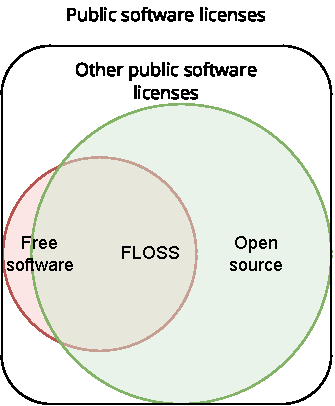
\includegraphics[scale=1.5]{figures/terms-diagram.pdf}
	\caption{Public licenses in software engineering}
	\label{fig:terms}
\end{figure}

% free vs open
Let us explore further the differences and similarities between open source and free software at the software engineering level of public licenses. This is a crucial step since we can see from the approximation in \hyperref[fig:terms]{Figure 1.1} that the majority of public software licenses are either open source, free software or both. We glanced over the free software definition in the first section of \hyperref[intro]{Chapter 1}. Open Source Initiative defines open-source licenses in the Open Source Definition briefly in the following way \citep{osi:licenselist}:
\begin{quote}
	''Open source licenses are licenses that comply with the Open Source Definition - in brief, they allow software to be freely used, modified, and shared.''
\end{quote}
Like the FSF with free software, OSI has the final word on what passes as open source and what does not. For example a new public software license will not classify as free software nor open source until the corresponding organization has acknowledged the public software license as either free software, open source or neither. If a public software license is accepted by both FSF and OSI it will fall under the term FLOSS. If a public software license gets accepted by neither of the organization or it gets rejected by both organizations it will fall under ''Other public software licenses'' in the \hyperref[fig:terms]{Figure 1.1}. In general the strong copyleft free software license requirements are considered more strict than the open source license requirements. For the sake of perspective we could simplify the differences like so: free software requires the redistributions of the licensed software to be open as well but open source licenses do not usually require this. The terms free software and open source are in general often misunderstood or just thought of as FLOSS collectively because the terms have a hard time conveying their paradigms in the natural language. One would not think free software does not mean software free of charge nor would one think that open source allows closed source redistributions of the licensed software. We will glance over the impacts on the industry of these two terms in \hyperref[discussion]{Chapter 4}.

% define public liceneses in se
With the context laid out in this chapter let us define public licenses in software engineering for the purpose of this study: Public software licenses are copyright licenses where the licensees are not limited and the copyright license in question is meant be used in licensing software source code. This helps us create the search strings and find the relevant literature for this thesis. This also helps us exclude public licenses regarding documentation, media and all other non-software targeted public licenses.

% acknowledge the topic is complex
The quest to categorize every public software license under some paradigm objectively is a complex one and cannot be comprehensively answered in a single paragraph. Therefore it is essential to continue taking the correct steps towards incresing the scientific understanding and providing the industry with examples, standards and processes to follow. However, as the following chapters reveal, a significant amount of effort is still being spent on solving the same problem multiple times, rather than building on existing knowledge and finding the next problem to solve. This thesis aims to contribute to mitigating this challenge by providing a rigorous analysis of the current state of the field. As the knowledge, conventions, and terminology take shape,we can look forward to reaching a state where less effort is spent on defining concepts and more on practical problem-solving.